% Experiments for the Introspective Verification paper.
% Style: plain, direct; no em-dashes; minimal colons/quotes; no anthropomorphic verbs.
% Numbers: LVH / GenPRM (greedy) rows from the local runs; other ProcessBench rows
% (Math-Shepherd, RLHFlow, Skywork, EurusPRM, PRM800K, Dyve, GPT-4o, GenPRM Maj@8)
% are from GenPRM (arXiv:2504.00891) Table 1, itself built on ProcessBench.

\section{Experiments}
\label{sec:experiments}

We test one claim: a discriminative read of the backbone's hidden states matches a generative process reward model on step level verification at a fraction of its cost. We recall the operation under test, describe the protocol, and then report the 1.5B result, the fusion with a generative verifier, the behavior at 7B, and the compute accounting.

\subsection{The head under test}
\label{sec:exp-head}

We evaluate the introspective verdict head of \Cref{sec:method}, which we abbreviate LVH in the tables. It scores a step in one forward pass by summing a linear readout on the final layer and an MLP readout on an automatically selected intermediate layer $\ell^\star$ (\Cref{eq:head}), with the backbone LoRA adapted on step labels, and with no decoding and no code execution. For DeepSeek-R1-Distill-Qwen the selection returns $\ell^\star=20$ of $28$, near seventy percent of the depth, and we use this layer at both scales.

\subsection{Setup}
\label{sec:exp-setup}

\paragraph{Benchmark and metric.} We evaluate on ProcessBench \citep{zheng2024processbench}, which asks a verifier to locate the first incorrect step in a solution, or to report that every step is correct. The benchmark has four subsets of increasing difficulty, GSM8K, MATH, OlympiadBench, and OmniMATH. The metric for each subset is the localization F1, the harmonic mean of two accuracies, the accuracy on erroneous solutions where the predicted first error must match the labeled step, and the accuracy on correct solutions where the verifier must predict no error. We report the four subsets and their mean.

\paragraph{Backbones.} We use DeepSeek-R1-Distill-Qwen at the 1.5B and the 7B scale as the verifier backbone. Both have 28 transformer layers, so $\ell^\star=20$ is the same relative depth at both scales. Training and inference run on a single V100 class GPU in a few hours, in bf16 or fp16, with gradient checkpointing so the backbone and the two heads stay within one device.

\paragraph{Training labels.} Supervision is the step level Yes/No labels released with GenPRM \citep{zhao2025genprm}, which come from math model trajectories with relative progress estimation. The method uses only these labels, not the GenPRM model. We train on the order of eight thousand conversations.

\paragraph{Baselines.} We compare against the process reward models tabulated on ProcessBench and by GenPRM. These are the classification models Math-Shepherd-PRM-7B \citep{wang2023mathshepherd}, RLHFlow-PRM-8B, Skywork-PRM-7B, and EurusPRM-Stage2, the discriminative Qwen2.5-Math-7B model trained on PRM800K \citep{lightman2023lets, zhang2025lessons}, the adaptive Dyve at 14B \citep{zhong2025dyve}, and GPT-4o used as a critic without a process reward model. We also compare against GenPRM at the matching 1.5B and 7B size, in both its greedy single pass form and its eight sample majority vote form. The greedy GenPRM rows are measured in our environment with the official incremental protocol, and reproduce the released scores; the remaining external rows are from GenPRM Table 1.

\subsection{An intermediate layer carries the signal}
\label{sec:exp-layer}

Before the benchmark we locate where step correctness is decodable. We freeze the 7B backbone, take the last token hidden state of each step at eight candidate layers, and fit a balanced logistic probe on step correctness. \Cref{tab:layersweep} reports two quantities per layer, the step level separability as the area under the ROC curve, and the localization F1 of the probe. Both peak at the same place. As a probe, the intermediate layer nine below the output, at about seventy percent of the depth, is the most separable on both measures, 0.915 AUC and 44.2 F1, and separability declines toward the final layer and toward the middle of the network. In raw separability the intermediate layer, not the final layer, is where step correctness reads out most cleanly. This sweep is exactly the automatic selection of \Cref{alg:select} run on the 7B backbone, so the head reads from the layer this procedure returns rather than from a hand chosen one, and \Cref{fig:layersweep} plots the full curve.

\begin{table}[t]
  \centering
  \caption{Per layer probe separability on the frozen 7B backbone. Layer $-k$ is $k$ layers below the output; relative depth is the position among the 28 transformer layers. Step correctness is most separable, on both the step level AUC and the probe localization F1, at the intermediate layer nine below the output, near seventy percent of the depth, and separability falls off toward the final layer.}
  \label{tab:layersweep}
  \begin{tabular}{lcccccccc}
    \toprule
    Layer (from top) & $-1$ & $-3$ & $-5$ & $-7$ & $-9$ & $-11$ & $-13$ & $-15$ \\
    Relative depth & 100\% & 93\% & 86\% & 79\% & \textbf{71\%} & 64\% & 57\% & 50\% \\
    \midrule
    Step AUC        & 0.907 & 0.905 & 0.896 & 0.910 & \textbf{0.915} & 0.904 & 0.889 & 0.867 \\
    Localization F1 & 42.2 & 38.7 & 39.4 & 37.7 & \textbf{44.2} & 41.2 & 33.9 & 31.2 \\
    \bottomrule
  \end{tabular}
\end{table}

\subsection{The residual form}
\label{sec:exp-ablation}

The head reads the intermediate layer, where step correctness is most separable (\Cref{tab:layersweep}), and adds a final layer readout for calibration. \Cref{tab:ablation} trains the two readouts separately and together at the same budget to show what each contributes. A trained readout is not the same as a raw probe, and the two roles are different. The final layer readout is trained to emit the verdict itself, so as a standalone readout it is well calibrated, 58.6 mean F1, even though the final layer's raw separability is the lower of the two (\Cref{tab:layersweep}). The intermediate readout alone is discriminative but poorly calibrated, 54.4, since nothing anchors the scale of its scores. The residual head keeps the intermediate layer's discrimination and the final layer's calibration. It dominates the intermediate readout on every subset, matches the calibrated final readout in the mean, and exceeds it on the two proof heavy subsets, OlympiadBench and OmniMATH, by 1.4 and 1.2 points, where discrimination matters most. The value of the residual form is therefore not a higher mean but a redistribution of accuracy toward the harder subsets at no cost elsewhere.

\begin{table}[t]
  \centering
  \caption{Contribution of each readout at 1.5B, trained at the same full budget (8000 conversations, 15000 steps), localization F1. The final readout is trained to be the verdict, so on its own it is well calibrated; the intermediate readout is discriminative but uncalibrated; the residual head keeps both and exceeds the calibrated final readout on the two proof heavy subsets. This is a trained readout comparison and is distinct from the raw separability of \Cref{tab:layersweep}. The residual mean, 58.5, matches the headline 58.1 of \Cref{tab:pb} within run to run noise.}
  \label{tab:ablation}
  \begin{tabular}{lccccc}
    \toprule
    Trained readout & GSM8K & MATH & Olympiad & OmniMATH & Mean \\
    \midrule
    Final layer only        & \textbf{67.9} & \textbf{64.3} & 51.6 & 50.7 & \textbf{58.6} \\
    Intermediate layer only & 59.7 & 58.2 & 49.9 & 49.7 & 54.4 \\
    Residual (both)         & 65.3 & 63.8 & \textbf{53.0} & \textbf{51.9} & 58.5 \\
    \bottomrule
  \end{tabular}
\end{table}

\subsection{Introspection matches a generative verifier at 1.5B}
\label{sec:exp-main}

\Cref{tab:pb} (top panel) reports the full ProcessBench result at the 1.5B scale. The introspective head reaches 58.1 mean F1 from a single forward pass. This exceeds every classification process reward model in the table, including models at 7B and 8B scale, and it exceeds the discriminative PRM800K model at 7B and Dyve at 14B. It also exceeds the same size generative model GenPRM-1.5B in its greedy form, 58.1 against 57.2, while reading the solution once rather than decoding a critique and calling an interpreter. The score approaches the 61.9 of GPT-4o, a much larger general model used as a critic. A stronger but much costlier configuration of the generative model, eight sample majority voting, reaches 63.4; sampling and voting are orthogonal and could be applied to either verifier, so we do not treat their absence as an advantage of the head. The per subset pattern is informative. The head leads on GSM8K by a wide margin, stays close on MATH and OlympiadBench, and is weakest on OmniMATH, the proof heavy subset where a cheap ranking signal is hardest to extract.

\begin{table}[t]
  \centering
  \caption{ProcessBench localization F1. \emph{Top panel:} 1.5B scale on the full benchmark. \emph{Bottom panel:} 7B scale on 120 case slices. External rows are from ProcessBench \citep{zheng2024processbench} and GenPRM \citep{zhao2025genprm} Table 1; GenPRM greedy rows are measured in our environment with the official incremental protocol and reproduce the released scores. The introspective head (LVH) uses one forward pass, with no generation and no code execution. LVH-7B standalone uses the unsupervised per domain calibration of \Cref{sec:exp-7b}; the fusion row is the honest leave one domain out combination.}
  \label{tab:pb}
  \begin{tabular}{llccccc}
    \toprule
    & Method & GSM8K & MATH & Olympiad & OmniMATH & Mean \\
    \midrule
    \multirow{10}{*}{\rotatebox{90}{\textbf{1.5B} \; full}}
    & Math-Shepherd-PRM-7B      & 47.9 & 29.5 & 24.8 & 23.8 & 31.5 \\
    & RLHFlow-PRM-8B            & 38.8 & 33.8 & 16.9 & 16.9 & 26.6 \\
    & Skywork-PRM-7B           & 70.8 & 53.6 & 22.9 & 21.0 & 42.1 \\
    & EurusPRM-Stage2          & 47.3 & 35.7 & 21.2 & 20.9 & 31.3 \\
    & Qwen2.5-Math-7B-PRM800K  & 68.2 & 62.6 & 50.7 & 44.3 & 56.5 \\
    & Dyve-14B                 & 68.5 & 58.3 & 49.0 & 47.2 & 55.8 \\
    & GPT-4o (critic, no PRM)  & 79.2 & 63.6 & 51.4 & 53.5 & 61.9 \\
    & GenPRM-1.5B (greedy)     & 52.8 & 66.6 & 55.1 & 54.5 & 57.2 \\
    & GenPRM-1.5B (Maj@8)      & 51.3 & 74.4 & 65.3 & 62.5 & 63.4 \\
    & \textbf{LVH-1.5B (ours, one pass)} & \textbf{65.1} & 61.3 & 53.5 & 52.4 & \textbf{58.1} \\
    \midrule
    \multirow{3}{*}{\rotatebox{90}{\textbf{7B}}}
    & GenPRM-7B (greedy)       & 83.4 & 80.0 & 72.3 & 71.5 & 76.8 \\
    & LVH-7B (ours, one pass)  & 72.5 & 76.6 & 68.1 & 57.0 & 68.5 \\
    & \textbf{LVH $\oplus$ GenPRM-7B (fusion)} & \textbf{83.4} & \textbf{81.5} & \textbf{73.2} & \textbf{71.5} & \textbf{77.4} \\
    \bottomrule
  \end{tabular}
\end{table}

\subsection{Where the head succeeds and fails}
\label{sec:exp-erranalysis}

\Cref{tab:perdomain} splits the localization F1 into its parts, the accuracy on erroneous solutions and on correct ones, and on the error side the fractions where the head places the error correctly, flags the wrong step, or misses the error. The failure mode shifts with difficulty. On GSM8K the head mostly misses errors, 25.1 percent, and rarely mislocates them, 21.7 percent. On OmniMATH it almost never misses, 7.8 percent, but flags the wrong step 44.3 percent of the time. On easy problems the head fails by overlooking an error, and on hard problems it detects that something is wrong but cannot place it. The step level AUC stays high across subsets, from 0.866 to 0.891, so the difficulty is in localization, not in telling an error step from a correct one in isolation. Two structural factors deepen this localization gap (\Cref{fig:lengthpos}). Localization F1 falls with solution length, for example on MATH from 70.1 on short solutions to 47.0 on the longest, and localization accuracy falls the later the true error sits, from 63.6 percent at the first step to 33.1 percent at the fifth or later. Both hold because the head must first read every earlier step as correct. Threshold and calibration analyses are in \Cref{app:extended}.

\begin{table}[t]
  \centering
  \caption{Per domain error budget for LVH-1.5B, at the tuned threshold. Wrong step and Missed are the fractions of erroneous solutions where the head flags the wrong step or reports no error. Step AUC pools per step scores against per step labels.}
  \label{tab:perdomain}
  \begin{tabular}{lcccccc}
    \toprule
    Subset & Step AUC & F1 & Error acc. & Correct acc. & Wrong step \% & Missed \% \\
    \midrule
    GSM8K    & 0.889 & 65.1 & 53.1 & 83.9 & 21.7 & 25.1 \\
    MATH     & 0.891 & 61.3 & 51.0 & 76.8 & 38.6 & 10.4 \\
    Olympiad & 0.876 & 53.5 & 46.7 & 62.5 & 43.6 & \phantom{0}9.7 \\
    OmniMATH & 0.866 & 52.4 & 48.0 & 57.7 & 44.3 & \phantom{0}7.8 \\
    \bottomrule
  \end{tabular}
\end{table}

\begin{figure}[t]
  \centering
  \begin{subfigure}{0.49\linewidth}\centering
  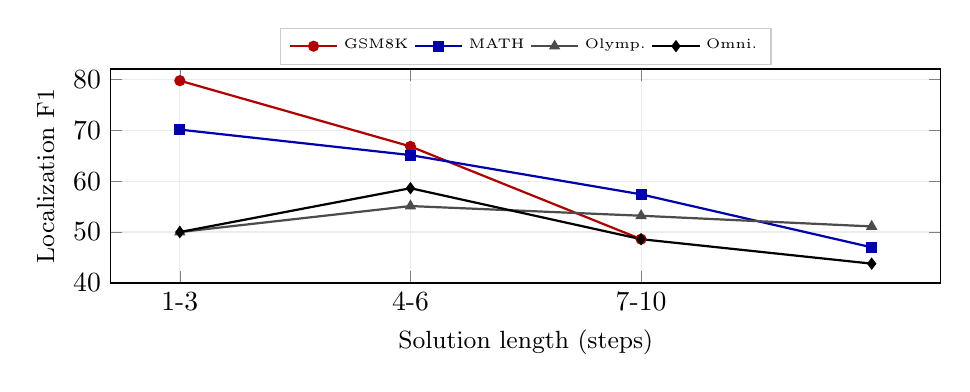
\begin{tikzpicture}
    \begin{axis}[width=\linewidth, height=4.3cm, symbolic x coords={1-3,4-6,7-10,11+}, xtick=data,
      xlabel={Solution length (steps)}, xlabel style={font=\small}, ylabel={Localization F1}, ylabel style={font=\small},
      ymin=40, ymax=82, grid=major, grid style={gray!15},
      legend style={font=\tiny, at={(0.5,1.02)}, anchor=south, legend columns=4, draw=gray!40}]
    \addplot[thick,mark=*,mark size=1.6pt,red!70!black] coordinates {(1-3,79.7)(4-6,66.8)(7-10,48.6)};
    \addplot[thick,mark=square*,mark size=1.6pt,blue!70!black] coordinates {(1-3,70.1)(4-6,65.1)(7-10,57.4)(11+,47.0)};
    \addplot[thick,mark=triangle*,mark size=1.6pt,gray!60!black] coordinates {(1-3,50.0)(4-6,55.1)(7-10,53.2)(11+,51.1)};
    \addplot[thick,mark=diamond*,mark size=1.6pt,black] coordinates {(1-3,50.0)(4-6,58.6)(7-10,48.6)(11+,43.8)};
    \legend{GSM8K,MATH,Olymp.,Omni.}
    \end{axis}
  \end{tikzpicture}
  \subcaption{F1 by solution length.}\label{fig:length}
  \end{subfigure}\hfill
  \begin{subfigure}{0.49\linewidth}\centering
  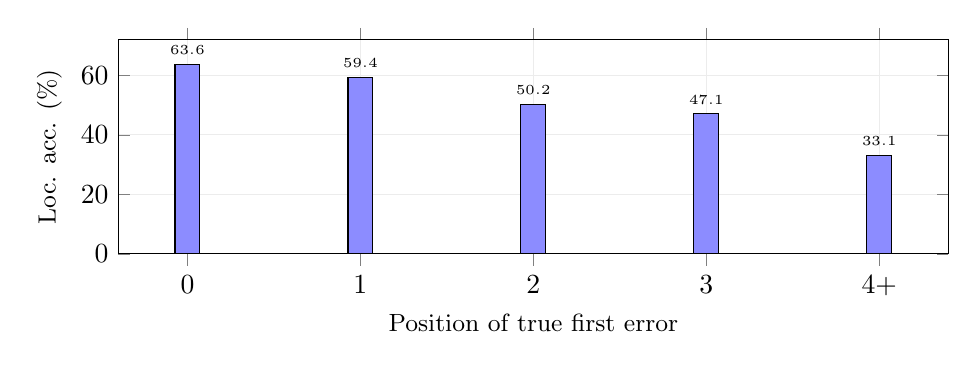
\begin{tikzpicture}
    \begin{axis}[width=\linewidth, height=4.3cm, ybar, bar width=9pt, symbolic x coords={0,1,2,3,4+}, xtick=data,
      xlabel={Position of true first error}, xlabel style={font=\small}, ylabel={Loc. acc. (\%)}, ylabel style={font=\small},
      ymin=0, ymax=72, grid=major, grid style={gray!15},
      nodes near coords, nodes near coords style={font=\tiny}]
    \addplot[fill=blue!45] coordinates {(0,63.6)(1,59.4)(2,50.2)(3,47.1)(4+,33.1)};
    \end{axis}
  \end{tikzpicture}
  \subcaption{Accuracy by error position.}\label{fig:errpos}
  \end{subfigure}
  \caption{Localization for LVH-1.5B degrades with solution length \textbf{(a)} and with a later error position \textbf{(b)}, because the head must first pass every earlier step.}
  \label{fig:lengthpos}
\end{figure}

\subsection{Introspection is complementary to generation}
\label{sec:exp-fusion}

The two signals read different evidence, so we test whether they combine. We form a logit space sum of the introspective reward and a generative verifier score, with a single weight and bias fixed on a held out MATH split and never on the test subsets. On matched 120 case slices of the four subsets, this fixed combination improves the mean localization F1 by 5.4 points over the greedy generative verifier alone. The gain is not a re-ranking of the same errors. The head recovers cases where a fluent but wrong step misleads the surface verdict, and the generative verifier keeps the cases where a written derivation is needed, so the sum is above either input. This is the practical form of the finding: an introspective read is not only cheap, it carries evidence that a generative verifier does not already have.

\subsection{At 7B, generation earns its cost, and introspection remains a near free add on}
\label{sec:exp-7b}

We repeat the study at 7B on 120 case slices in the bottom panel of \Cref{tab:pb}. Here the generative verifier is stronger, 76.8 mean F1, and the introspective head alone no longer matches it. Its raw logits carry a per domain offset at 7B, most visible on OlympiadBench, so we center them per domain with an unsupervised median shift estimated on the domain's own scores, with no labels. This raises the standalone head from 64.2 to 68.5 mean F1 (\Cref{app:calib}), but it is still short of the generative verifier, which marks the regime where generation is worth its cost. The head remains useful as an add on. The honest leave one domain out fusion, which never tunes on the domain it scores, improves MATH and OlympiadBench, does not lower any subset, and raises the mean from 76.8 to 77.4. This per domain centering assumes the test domain is known at inference; a domain agnostic global centering returns only the generative baseline of 76.8, so the gain depends both on this domain metadata and on the calibration itself (\Cref{app:calib}). The picture across scales gives a simple cost accuracy rule. At small scale the introspective head is Pareto optimal, matching or beating trained process reward models from one forward pass (\Cref{fig:pareto}). At large scale it is a near free add on to a generative process reward model, since one extra forward pass is negligible next to repeated decoding.

\Cref{fig:fusion} decomposes the 7B fusion by subset. It matches or beats the generative verifier everywhere and gains where the verifier has room, plus 1.5 on MATH and plus 0.9 on OlympiadBench, while it stays level on the subsets the verifier already handles. The complementarity is also visible case by case. \Cref{fig:agree} classifies the 480 shared cases by which verifier is right. The two agree on the outcome in 342 cases, both correct in 275 and both wrong in 67. Of the 138 where exactly one is right, the generative verifier is right more often, 98 against 40, which is why it is the stronger verifier at 7B, while the 40 cases the head uniquely fixes are what the fusion recovers. \Cref{app:cases} analyzes one case from each cell. The fusion is insensitive to the exact weight it places on the head, with a broad plateau of near optimal weights (\Cref{fig:fusionweight}).

\begin{figure}[t]
  \centering
  \begin{minipage}[b]{0.63\linewidth}\centering
    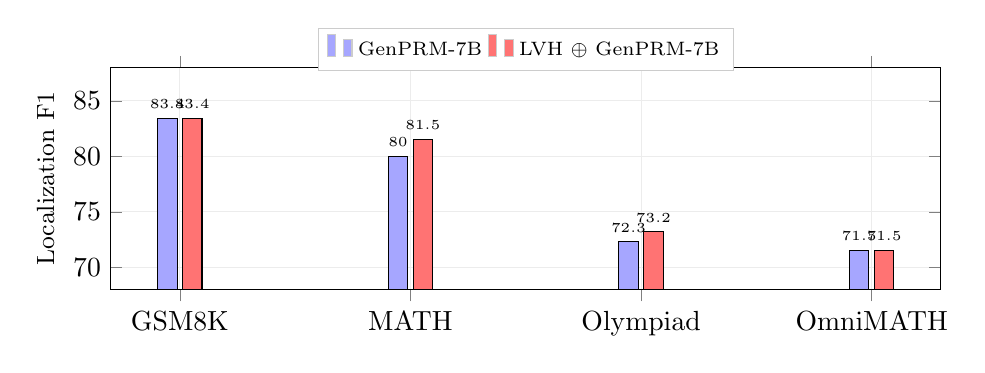
\begin{tikzpicture}
      \begin{axis}[
        width=\linewidth, height=4.4cm,
        ybar, bar width=7pt,
        symbolic x coords={GSM8K, MATH, Olympiad, OmniMATH},
        xtick=data, ymin=68, ymax=88, ylabel={Localization F1}, ylabel style={font=\small},
        legend style={at={(0.5,1.18)}, anchor=north, legend columns=2, font=\scriptsize, draw=gray!40},
        grid=major, grid style={gray!15},
        nodes near coords, nodes near coords style={font=\tiny},
        every node near coord/.append style={/pgf/number format/fixed, /pgf/number format/precision=1},
      ]
      \addplot[fill=blue!35] coordinates {(GSM8K,83.4)(MATH,80.0)(Olympiad,72.3)(OmniMATH,71.5)};
      \addplot[fill=red!55] coordinates {(GSM8K,83.4)(MATH,81.5)(Olympiad,73.2)(OmniMATH,71.5)};
      \legend{GenPRM-7B, LVH $\oplus$ GenPRM-7B}
      \end{axis}
    \end{tikzpicture}
    \subcaption{Fusion decomposition by subset.}\label{fig:fusion}
  \end{minipage}\hfill
  \begin{minipage}[b]{0.34\linewidth}\centering
    \small
    \begin{tabular}{lcc}
      \toprule
      & \multicolumn{2}{c}{Generative} \\
      Head & correct & wrong \\
      \midrule
      correct & 275 & \textbf{40} \\
      wrong   & \textbf{98} & 67 \\
      \bottomrule
    \end{tabular}
    \vspace{2mm}
    \subcaption{Agreement on 480 cases.}\label{fig:agree}
  \end{minipage}
  \caption{Complementarity at 7B. \textbf{(a)} The honest leave one domain out fusion matches or beats the generative verifier on every subset, gaining where it has room. \textbf{(b)} The head uniquely fixes 40 cases the generative verifier gets wrong, which is what the fusion recovers.}
  \label{fig:complement}
\end{figure}

\subsection{Compute accounting}
\label{sec:exp-compute}

The cost gap is the point of the method, so we make it explicit on two axes, token compute and measured wall clock. The introspective head reads the solution once and produces every step reward in that single forward pass, with no autoregressive decoding and no interpreter call. A single greedy pass of the same size generative verifier reads the same solution and then decodes a critique, and it also runs code. On our 7B outputs the critique is about 3.5 times as many tokens as the solution, measured over 480 cases. In token compute, reading is one prefill while decoding is one forward pass per generated token, so a single greedy generative pass costs about four times the token compute of the head, and the head spends about one quarter of it. Wall clock makes the gap larger, because the decoded tokens are produced one forward pass at a time while the head reads all tokens in a single parallel prefill. On one V100 at 7B, the greedy generative verifier takes a median of 31 seconds per solution end to end including code execution, while the introspective head scores the same solution in about 1 second unbatched, a median speedup near 32 times. We compare against the greedy verifier throughout, since sampling and voting would raise the cost of both verifiers. The head therefore sits at a different point on the cost accuracy curve. It reaches a mean F1 in the range of a strong single pass generative verifier while spending the compute of a single read.

\begin{figure}[t]
  \centering
  \begin{minipage}[b]{0.49\linewidth}\centering
    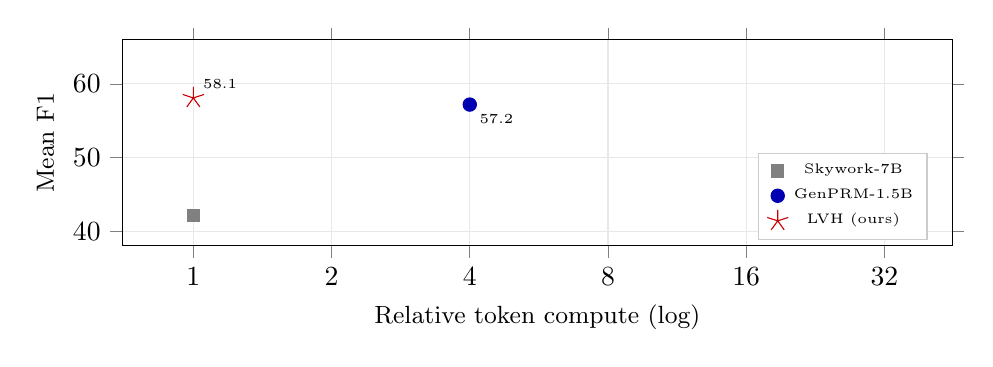
\begin{tikzpicture}
      \begin{axis}[
        width=\linewidth, height=4.2cm,
        xmode=log, log basis x=2,
        xtick={1,2,4,8,16,32}, xticklabels={1,2,4,8,16,32},
        xlabel={Relative token compute (log)}, xlabel style={font=\small},
        ylabel={Mean F1}, ylabel style={font=\small},
        ymin=38, ymax=66, xmin=0.7, xmax=45,
        grid=both, grid style={gray!18}, tick align=outside,
        legend pos=south east, legend style={font=\tiny, fill=white, draw=gray!40},
      ]
      \addplot[only marks, mark=square*, mark size=2.2pt, color=gray] coordinates {(1,42.1)};
      \addlegendentry{Skywork-7B}
      \addplot[only marks, mark=*, mark size=2.4pt, color=blue!70!black] coordinates {(4,57.2)};
      \addlegendentry{GenPRM-1.5B}
      \addplot[only marks, mark=star, mark size=4pt, color=red!80!black] coordinates {(1,58.1)};
      \addlegendentry{LVH (ours)}
      \node[anchor=south west, font=\tiny] at (axis cs:1,58.1) {58.1};
      \node[anchor=north west, font=\tiny] at (axis cs:4,57.2) {57.2};
      \end{axis}
    \end{tikzpicture}
    \subcaption{Cost--accuracy frontier (1.5B).}\label{fig:pareto}
  \end{minipage}\hfill
  \begin{minipage}[b]{0.49\linewidth}\centering
    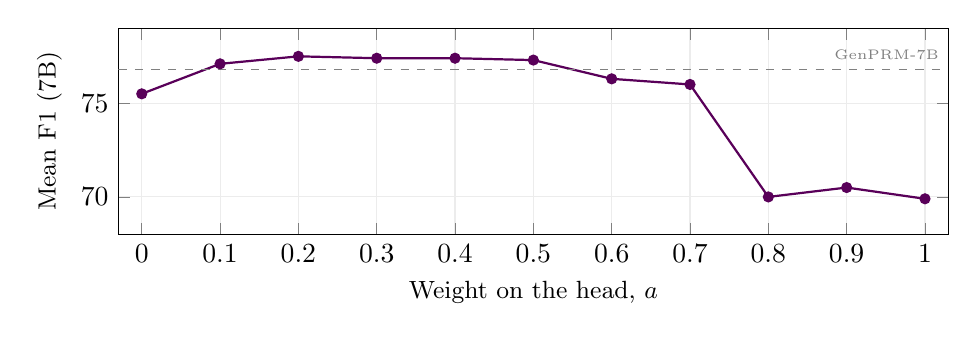
\begin{tikzpicture}
      \begin{axis}[width=\linewidth, height=4.2cm, xlabel={Weight on the head, $a$}, xlabel style={font=\small},
        ylabel={Mean F1 (7B)}, ylabel style={font=\small},
        xmin=-0.03, xmax=1.03, ymin=68, ymax=79, grid=major, grid style={gray!15}]
      \addplot[thick, mark=*, mark size=1.6pt, color=violet!70!black] coordinates {(0,75.5)(0.1,77.1)(0.2,77.5)(0.3,77.4)(0.4,77.4)(0.5,77.3)(0.6,76.3)(0.7,76.0)(0.8,70.0)(0.9,70.5)(1.0,69.9)};
      \draw[dashed,gray] (axis cs:-0.03,76.8)--(axis cs:1.03,76.8);
      \node[anchor=south east,font=\tiny,gray] at (axis cs:1.03,76.8) {GenPRM-7B};
      \end{axis}
    \end{tikzpicture}
    \subcaption{Fusion is robust to the mixing weight.}\label{fig:fusionweight}
  \end{minipage}
  \caption{\textbf{(a)} At 1.5B the introspective head (star) reaches higher mean F1 than a greedy generative pass at about one quarter of its token compute (GPT-4o, 61.9, omitted as a much larger model). \textbf{(b)} The 7B fusion mean F1 against the weight $a$ on the head; a broad plateau spans $a\in[0.1,0.5]$, so the fusion is insensitive to the exact weight.}
  \label{fig:costfusion}
\end{figure}

\subsection{Honest notes}
\label{sec:exp-honest}

The clearest limitation of the cheap head is OmniMATH, the proof heavy subset. Its per step separability is the lowest of the four subsets, a step level AUC of 0.866 (\Cref{tab:perdomain}), and the sharper limit is that the head over flags correct proofs and mislocates errors on long solutions, which is why it is weakest there and why the fusion defers to the generative verifier on it (\Cref{app:omnimath}). The per domain median shift that the 7B fusion uses is a scale specific trick, not a component of the method, and we explain in \Cref{app:calib} why the 7B head needs it and the 1.5B head does not.
